\documentclass[%
    school=etsisi,%
    type=pfg,%
    degree=61CI,%
]{upm-report}

% La clase no tiene tipo "pfa" nativo; lo redefinimos tras cargarla.
\renewcommand{\reporttype}{Proyecto Fin de Asignatura}
\renewcommand{\reporttypeabbr}{PFA}
% Suprimir el abstract en inglés (solo se usa el resumen en español)
\renewcommand\makeabstract{}

%%%%%%%%%%%%%%%%%%%%%%%%%%%%%%%%%%%%%%%%%%%%%%%%%%%%%%%%%%%%%%%%%%%%%%%%
% TÍTULO, AUTOR Y DIRECTOR
%
\title{Implementación del procesador Intel~4004 en VHDL sobre FPGA Basys~3 Artix-7}
\subject{Programación de Hardware Reconfigurable}
\author{%
    Ander Regidor Barrante\\
    Iván Serrano Prieto\\
    Maria José García-Prieto Castells\\
    Elena Esparza Baña%
}
\bibauthor{Regidor Barrante, A.; Serrano Prieto, I.; García-Prieto Castells, M.\,J.; Esparza Baña, E.}
\director{Vicente A. García Alcántara}

%%%%%%%%%%%%%%%%%%%%%%%%%%%%%%%%%%%%%%%%%%%%%%%%%%%%%%%%%%%%%%%%%%%%%%%%
% RESUMEN Y ABSTRACT
%
\abstract{spanish}{
    Este trabajo recoge el diseño e implementación en \acrshort{vhdl} del
    procesador \acrshort{cpu} Intel~4004, el primer microprocesador comercial
    de la historia, sobre una placa de desarrollo Basys~3 equipada con una
    \acrshort{fpga} Artix-7 de Xilinx.

    El diseño sigue fielmente la especificación técnica original del Intel~4004,
    organizando el hardware en bloques funcionales equivalentes a los del
    diagrama oficial: ruta de datos, unidad de control, pila de direcciones,
    banco de registros y lógica de interfaz con memoria externa.  Cada bloque
    se describe en esta memoria junto con las decisiones de implementación que
    lo justifican.

    % TODO: completar con resultados de síntesis, verificación y conclusiones
    % cuando estén disponibles.

    \bigskip
    \begin{center}
        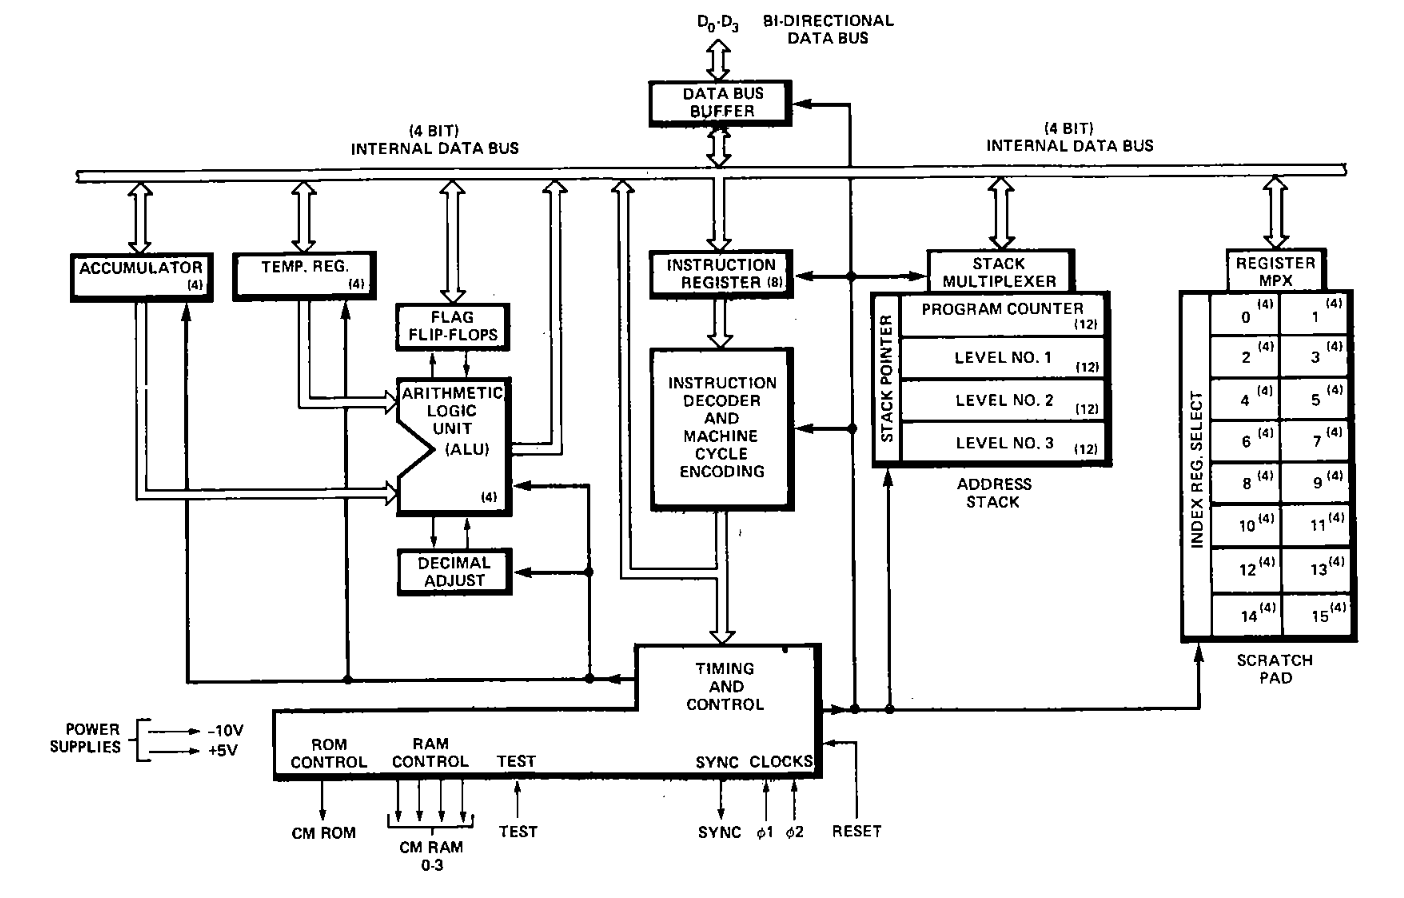
\includegraphics[width=0.88\textwidth]{diagrama}\\[0.6em]
        {\small\textit{Diagrama de bloques del procesador Intel~4004}}
    \end{center}
}
\keywords{spanish}{
    VHDL;
    Intel 4004;
    FPGA;
    Artix-7;
    Arquitectura de computadores
}

%%%%%%%%%%%%%%%%%%%%%%%%%%%%%%%%%%%%%%%%%%%%%%%%%%%%%%%%%%%%%%%%%%%%%%%%
% GLOSARIO Y ACRÓNIMOS
%
\newacronym{vhdl}{VHDL}{\textit{Very High Speed Integrated Circuit Hardware Description Language}}
\newacronym{fpga}{FPGA}{\textit{Field Programmable Gate Array}}
\newacronym{cpu}{CPU}{Unidad Central de Proceso}
\newacronym{alu}{ALU}{Unidad Aritmético-Lógica}
\newacronym{ir}{IR}{Registro de Instrucción}
\newacronym{pc}{PC}{\textit{Program Counter}}
\newacronym{bcd}{BCD}{\textit{Binary Coded Decimal}}
\newacronym{phr}{PHR}{Programación de Hardware Reconfigurable}
\newacronym{ff}{FF}{\textit{Flip-Flop}}
\newacronym{fsm}{FSM}{\textit{Finite State Machine}}
\newacronym{oe}{OE}{\textit{Output Enable}}
\newacronym{bram}{BRAM}{\textit{Block RAM}}

\newglossaryentry{bus-interno}{
    name=bus interno,
    description={Bus de datos de 4~bits que interconecta todos los bloques
        funcionales internos de la CPU. Equivale al bus \textit{BUS} del
        diagrama de la especificación Intel~4004}
}
\newglossaryentry{nibble}{
    name=nibble,
    description={Grupo de 4~bits. La CPU Intel~4004 opera de forma nativa
        con nibbles al ser un procesador de 4~bits}
}
\newglossaryentry{scratchpad}{
    name=scratchpad,
    description={Banco de 16~registros de 4~bits internos a la CPU,
        denominados R0--R15, que el programador puede usar como registros
        de propósito general}
}
\newglossaryentry{stack}{
    name=pila de direcciones,
    description={Estructura de tres niveles de 12~bits cada uno que almacena
        las direcciones de retorno de las llamadas a subrutina}
}

% Subtítulo de fichero VHDL bajo cada subsección
\newcommand{\vhdlfile}[1]{%
    \par\noindent{\small\sffamily\color{gray}Fichero: \texttt{#1}}\par\smallskip
}

\addbibresource{references.bib}

\begin{document}

% ======================================================================
\chapter{Introducción}
\label{ch:introduccion}
% ======================================================================

% TODO: redactar la introducción completa.

El Intel~4004, lanzado en 1971, fue el primer \acrfull{cpu} comercial
integrado en un único circuito integrado.  Con una arquitectura de 4~bits,
700~kHz de frecuencia máxima y apenas 2300~transistores, supuso el punto de
partida de la industria del microprocesador.

El objetivo de este proyecto, enmarcado en la asignatura
\acrfull{phr} del Grado en Ingeniería de Computadores de la
\textit{Escuela Técnica Superior de Ingeniería de Sistemas Informáticos} de la
\textit{Universidad Politécnica de Madrid}, es implementar fielmente este
procesador en \acrshort{vhdl} y sintetizarlo sobre una \acrshort{fpga}
Artix-7 Basys~3.

\section{Objetivos}

El objetivo principal es implementar el procesador Intel~4004 de forma
funcional en \acrshort{vhdl}, verificar su correcto funcionamiento mediante
simulación y programarlo sobre la plataforma hardware Basys~3.  Se establecen
los siguientes objetivos específicos:

\begin{enumerate}
    \item Estudiar y comprender la especificación técnica original del
        Intel~4004.
    \item Diseñar la arquitectura en \acrshort{vhdl} dividida en bloques
        funcionales fiel al diagrama de la especificación.
    \item Verificar cada bloque de forma individual mediante \textit{testbenches}.
    \item Sintetizar e implementar el diseño completo sobre la Basys~3 Artix-7.
    \item Documentar todas las decisiones de diseño en esta memoria.
\end{enumerate}

\section{Estructura de la memoria}

% TODO: completar cuando la estructura definitiva esté cerrada.

El capítulo~\ref{ch:estado-cuestion} describe brevemente la arquitectura del
Intel~4004 y el marco tecnológico del proyecto.  El
capítulo~\ref{ch:metodologia} presenta la metodología de diseño seguida.
El capítulo~\ref{ch:diseno} contiene el grueso técnico del trabajo: la
estructura del código \acrshort{vhdl} y la descripción razonada de cada
bloque.  Los capítulos sucesivos, que se irán completando conforme avance el
proyecto, recogerán la verificación, la implementación sobre \acrshort{fpga}
y las conclusiones.

% ======================================================================
\chapter{Estado de la cuestión}
\label{ch:estado-cuestion}
% ======================================================================

% TODO: redactar esta sección.

\section{El procesador Intel 4004}

El Intel~4004 fue diseñado por Federico Faggin, Marcian Hoff, Stanley Mazor
y Masatoshi Shima para la calculadora Busicom.  Su arquitectura define un
conjunto de instrucciones de 46~operaciones con palabras de instrucción de
8~bits (o 16~bits para instrucciones de dos ciclos), un bus de datos
bidireccional de 4~bits y una frecuencia de operación de hasta 740~kHz.

Las características principales de su arquitectura son las siguientes:
un bus de datos externo de 4~bits (D0--D3); un bus de direcciones multiplexado
en el tiempo de 12~bits; un acumulador de 4~bits y su \acrshort{alu} asociada;
un banco de 16~registros internos (\gls{scratchpad}) de 4~bits organizables
en 8~pares de 8~bits; una \gls{stack} de tres niveles de 12~bits para llamadas
a subrutina; y lógica de control que genera las señales \texttt{SYNC},
\texttt{CM-ROM} y \texttt{CM-RAM} para la coordinación con la memoria externa.

\section{Herramientas utilizadas}

El flujo de diseño empleado en el proyecto se apoya en las siguientes
herramientas: \textit{Vivado Design Suite} de Xilinx como entorno de síntesis
e implementación; \acrshort{vhdl}-93 como lenguaje de descripción hardware; y
la placa Basys~3 (Artix-7 XC7A35T) como destino hardware.

% ======================================================================
\chapter{Metodología}
\label{ch:metodologia}
% ======================================================================

% TODO: desarrollar según las transparencias de la asignatura.

El proyecto sigue la metodología de diseño presentada en la asignatura
\acrshort{phr}, que estructura el trabajo en las siguientes fases: análisis de
la especificación, diseño de la arquitectura \acrshort{vhdl}, verificación
funcional mediante simulación, síntesis e implementación, y verificación sobre
hardware.  En el momento de redactar esta memoria el proyecto se encuentra en
la fase de diseño.

\bigskip
\begin{center}
    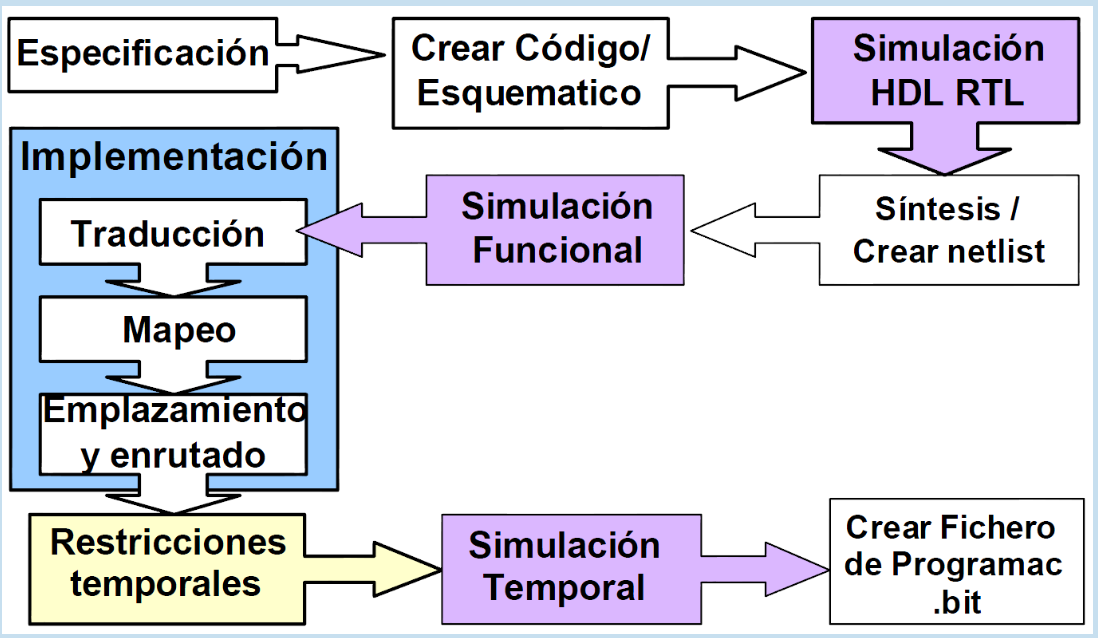
\includegraphics[width=0.82\textwidth]{metodologia}\\[0.6em]
    {\small\textit{Fases de la metodología de diseño de la asignatura \acrshort{phr}}}
\end{center}

% ======================================================================
\chapter{Diseño}
\label{ch:diseno}
% ======================================================================

Este capítulo describe en detalle el diseño \acrshort{vhdl} del
procesador Intel~4004.  En primer lugar se expone la filosofía de organización
del código; a continuación se describen, bloque a bloque, cada uno de los
componentes que integran la \acrshort{cpu}.

% ----------------------------------------------------------------------
\section{Estructura del proyecto en código}
\label{s:estructura}
% ----------------------------------------------------------------------

\subsection{Filosofía de diseño: arquitectura estructural jerárquica}

Una de las primeras decisiones de diseño del proyecto fue adoptar una
\textbf{arquitectura puramente estructural} en todos los niveles de la
jerarquía.  Esto significa que cada bloque funcional se implementa
instanciando componentes de nivel inferior hasta llegar, en la base de la
jerarquía, a primitivas de \textit{flip-flop} individuales.

Esta decisión es intencionada y responde a varios criterios.  Primero,
permite que el mapeado de la herramienta de síntesis a recursos físicos de la
\acrshort{fpga} sea completamente predecible: cada \texttt{registro\_4b}
se convierte en cuatro \textit{flip-flops} \texttt{FDRE}, un bus de cuatro
bits en cuatro rutas de señal, etcétera.  Segundo, facilita la verificación
incremental: cada primitiva puede simularse de forma aislada antes de
integrarse en el bloque superior.  Tercero, se mantiene una correspondencia
directa entre el diagrama de bloques de la especificación original
del Intel~4004 y la jerarquía de ficheros \acrshort{vhdl}.

\subsection{Fichero raíz}
\vhdlfile{cpu\_4004\_top.vhd}

El fichero \texttt{cpu\_4004\_top.vhd} es el punto de integración de todo el
diseño.  En él se declaran todas las señales internas del
\gls{bus-interno} y de control, y se instancian todos los bloques funcionales
mediante cláusulas \texttt{port map}.  No contiene lógica funcional propia:
su única responsabilidad es ensamblar los componentes y cablear las señales
entre ellos.

La entidad \texttt{cpu\_4004\_top} expone exactamente los pines físicos del
chip Intel~4004 original en encapsulado DIP-16: los dos relojes en cuadratura
(\texttt{clk\_ph1}, \texttt{clk\_ph2}), la señal de reset, el pin
\texttt{test}, las salidas de control \texttt{sync}, \texttt{cm\_rom} y
\texttt{cm\_ram}, y el bus de datos bidireccional de 4~bits \texttt{D\_bus}.

\subsection{Paquete de constantes}
\vhdlfile{pkg\_4004.vhd}

Para evitar el uso de literales numéricos dispersos por el código y facilitar
posibles modificaciones futuras, se define el paquete \texttt{pkg\_4004} que
centraliza las constantes globales del diseño.

\begin{lstlisting}[language=VHDL, caption={Contenido del paquete \texttt{pkg\_4004}},
    label=lst:pkg4004]
constant BUS_W     : integer := 4;
constant BUS_CERO  : std_logic_vector(BUS_W-1 downto 0) := "0000";
constant BUS_ERROR : std_logic_vector(BUS_W-1 downto 0) := "XXXX";
\end{lstlisting}

La constante \texttt{BUS\_W} define el ancho del \gls{bus-interno}; todos los
vectores de datos de 4~bits del diseño se dimensionan con ella.
\texttt{BUS\_CERO} representa el bus en estado inactivo y \texttt{BUS\_ERROR}
se utiliza para señalizar colisiones de bus durante la simulación (véase
la sección~\ref{ss:bus-interno}).

% ----------------------------------------------------------------------
\clearpage
\section{Primitivas de hardware}
\label{s:primitivas}
% ----------------------------------------------------------------------

En la base de la jerarquía de diseño se encuentran tres primitivas
que representan los elementos de memoria más simples.

\subsection{\textit{Flip-flop} D con enable}
\label{ss:d-ff-en}
\vhdlfile{d\_ff\_en.vhd}

Es el elemento de memoria fundamental del diseño.  Prácticamente todos los
registros de la \acrshort{cpu} se construyen como matrices de instancias de
esta entidad.  Su comportamiento es el de un \acrfull{ff} de tipo~D síncrono
con reset asíncrono activo alto y señal de habilitación:

\begin{table}[H]
\centering
\caption{Puertos de la entidad \texttt{d\_ff\_en}}
\label{tab:d-ff-en}
\begin{tabularx}{\textwidth}{@{}llcX@{}}
\toprule
\textbf{Puerto} & \textbf{Dir.} & \textbf{Bits} & \textbf{Descripción} \\
\midrule
\texttt{clk}   & in  & 1 & Reloj del sistema; captura en flanco de subida \\
\texttt{reset} & in  & 1 & Reset asíncrono activo alto; pone \texttt{q} a~\texttt{'0'} \\
\texttt{en}    & in  & 1 & Habilitación síncrona; si \texttt{'0'}, el estado no cambia \\
\texttt{d}     & in  & 1 & Dato de entrada \\
\texttt{q}     & out & 1 & Salida del \acrshort{ff} \\
\bottomrule
\end{tabularx}
\end{table}

La arquitectura \texttt{Behavioral} implementa la lógica de forma directa: en
el proceso sensible a \texttt{clk} y \texttt{reset}, si se produce reset la
salida se lleva a \texttt{'0'} de forma asíncrona; en el flanco de subida del
reloj, si \texttt{en = '1'}, se captura el valor de \texttt{d}.  La
herramienta de síntesis mapea este patrón directamente sobre un primitivo
\texttt{FDRE} de la Artix-7.

\subsection{Registros de 4 y 12 bits}
\label{ss:registros}
\vhdlfile{registro\_4b.vhd, registro\_12b.vhd}

Ambos registros se implementan de forma idéntica mediante una sentencia
\texttt{GENERATE} que instancia $N$ copias de \texttt{d\_ff\_en} en paralelo,
siendo $N = 4$ para \texttt{registro\_4b} y $N = 12$ para
\texttt{registro\_12b}.  Su interfaz es equivalente a la de \texttt{d\_ff\_en}
salvo que los puertos de datos son vectores.

Esta estrategia de construcción mediante \texttt{GENERATE} es coherente con
la filosofía estructural del proyecto: la descripción del registro no contiene
ninguna inferencia de comportamiento; es literalmente la unión de $N$
biestables individuales instanciados mediante síntesis paramétrica.

\begin{table}[H]
\centering
\caption{Puertos del \texttt{registro\_4b} (análogos en \texttt{registro\_12b})}
\label{tab:registro-4b}
\begin{tabularx}{\textwidth}{@{}llcX@{}}
\toprule
\textbf{Puerto} & \textbf{Dir.} & \textbf{Bits} & \textbf{Descripción} \\
\midrule
\texttt{clk}   & in  & 1 & Reloj del sistema \\
\texttt{R}     & in  & 1 & Reset asíncrono activo alto \\
\texttt{E}     & in  & 1 & Enable síncrono de escritura \\
\texttt{D\_in} & in  & 4 (12) & Dato a cargar cuando \texttt{E = '1'} \\
\texttt{Q\_out}& out & 4 (12) & Dato almacenado \\
\bottomrule
\end{tabularx}
\end{table}

\subsection{\textit{Flip-flop} JK}
\label{ss:ff-jk}
\vhdlfile{flipflopJK.vhd}

Este \acrshort{ff} de tipo~JK se utiliza exclusivamente en el puntero de pila
(véase la sección~\ref{ss:puntero-stack}).  Se implementa con arquitectura
\texttt{FlujoDatos}: la salida complementada \texttt{notq} se obtiene como
\texttt{not~q\_aux}, y la lógica JK se codifica como un proceso sensible al
reloj y al reset.

\begin{table}[H]
\centering
\caption{Puertos de la entidad \texttt{flipflopJK}}
\label{tab:ff-jk}
\begin{tabularx}{\textwidth}{@{}llcX@{}}
\toprule
\textbf{Puerto} & \textbf{Dir.} & \textbf{Bits} & \textbf{Descripción} \\
\midrule
\texttt{j}    & in  & 1 & Entrada J del biestable \\
\texttt{k}    & in  & 1 & Entrada K del biestable \\
\texttt{r}    & in  & 1 & Reset asíncrono activo alto \\
\texttt{clk}  & in  & 1 & Reloj de captura (flanco de subida) \\
\texttt{q}    & out & 1 & Salida directa \\
\texttt{notq} & out & 1 & Salida complementada \\
\bottomrule
\end{tabularx}
\end{table}

% ----------------------------------------------------------------------
\section{Ruta de datos}
\label{s:ruta-datos}
% ----------------------------------------------------------------------

\subsection{Acumulador}
\label{ss:accumulator}
\vhdlfile{accumulator.vhd}

El acumulador es el registro central de la \acrshort{alu}: almacena el primer
operando y el resultado de toda operación aritmética o lógica.  Su
implementación en \acrshort{vhdl} es intencionadamente trivial: la entidad
\texttt{accumulator} no es más que una envoltura (\textit{wrapper}) sobre
\texttt{registro\_4b}.  Esto es así porque el acumulador del Intel~4004 no
tiene ninguna lógica especial asociada; su particularidad reside en el rol
que juega en la microarquitectura, no en su comportamiento interno.

\begin{table}[H]
\centering
\caption{Puertos de la entidad \texttt{accumulator}}
\label{tab:accumulator}
\begin{tabularx}{\textwidth}{@{}llcX@{}}
\toprule
\textbf{Puerto} & \textbf{Dir.} & \textbf{Bits} & \textbf{Descripción} \\
\midrule
\texttt{clk}     & in  & 1 & Reloj del sistema \\
\texttt{reset}   & in  & 1 & Reset asíncrono \\
\texttt{load\_en}& in  & 1 & Señal de escritura procedente de \texttt{timing\_and\_control} \\
\texttt{d\_in}   & in  & 4 & Dato a cargar (proviene del \gls{bus-interno}) \\
\texttt{q\_out}  & out & 4 & Contenido actual del acumulador (hacia la \acrshort{alu} y el bus) \\
\bottomrule
\end{tabularx}
\end{table}

El acumulador recibe el dato siempre del \gls{bus-interno} y vuelca su
contenido directamente a la entrada~A de la \acrshort{alu} y, cuando
\texttt{acc\_oe = '1'}, también al bus interno a través del multiplexor
central.

\subsection{Registro temporal}
\label{ss:temp-register}
\vhdlfile{temp\_register.vhd}

El registro temporal es estructuralmente idéntico al acumulador (igualmente
un \textit{wrapper} sobre \texttt{registro\_4b}).  Su función es almacenar el
segundo operando de la \acrshort{alu} durante los ciclos de ejecución: en la
fase~X1, el controlador carga en él el valor del \gls{scratchpad} que
corresponda al registro fuente de la instrucción; en la fase~X2, ese valor
pasa a la entrada~B de la \acrshort{alu}.

La separación en dos entidades distintas (\texttt{accumulator} y
\texttt{temp\_register}) responde a razones de legibilidad y trazabilidad con
la especificación, aunque su descripción \acrshort{vhdl} sea idéntica.

\subsection{Unidad Aritmético-Lógica}
\label{ss:alu}
\vhdlfile{alu.vhd}

La \acrfull{alu} es el bloque combinacional que realiza todas las operaciones
aritméticas y lógicas de la \acrshort{cpu}.  Su arquitectura
\texttt{Combinational} no contiene ningún elemento de memoria; el resultado
está disponible de forma continua en función de sus entradas.

\begin{table}[H]
\centering
\caption{Puertos de la entidad \texttt{alu}}
\label{tab:alu}
\begin{tabularx}{\textwidth}{@{}llcX@{}}
\toprule
\textbf{Puerto}   & \textbf{Dir.} & \textbf{Bits} & \textbf{Descripción} \\
\midrule
\texttt{A\_in}      & in  & 4 & Primer operando (salida del acumulador) \\
\texttt{B\_in}      & in  & 4 & Segundo operando (temp. register o ajuste decimal) \\
\texttt{carry\_in}  & in  & 1 & Acarreo de entrada (\texttt{flags\_out[0]}) \\
\texttt{op}         & in  & 3 & Código de operación (véase la tabla~\ref{tab:alu-ops}) \\
\texttt{result\_out}& out & 4 & Resultado de la operación \\
\texttt{carry\_out} & out & 1 & Acarreo de salida \\
\texttt{zero\_flag} & out & 1 & Activo si \texttt{result\_out = 0000} \\
\bottomrule
\end{tabularx}
\end{table}

La \acrshort{alu} soporta siete operaciones seleccionadas mediante el vector
de 3~bits \texttt{op}:

\begin{table}[H]
\centering
\caption{Operaciones de la \acrshort{alu}}
\label{tab:alu-ops}
\begin{tabularx}{\textwidth}{@{}clX@{}}
\toprule
\textbf{\texttt{op}} & \textbf{Operación} & \textbf{Descripción} \\
\midrule
\texttt{000} & ADD  & $A + B + C_{in}$ \\
\texttt{001} & SUB  & $A + \overline{B} + C_{in}$ (resta en complemento a~1, fiel al 4004) \\
\texttt{010} & AND  & $A$ \textsc{and} $B$ \\
\texttt{011} & OR   & $A$ \textsc{or} $B$ \\
\texttt{100} & XOR  & $A$ \textsc{xor} $B$ \\
\texttt{101} & PASS & Pasa~$A$ sin modificar (valor por defecto) \\
\texttt{110} & INC  & $A + 1$ \\
\bottomrule
\end{tabularx}
\end{table}

Internamente, los tres resultados de mayor coste (ADD, SUB, INC) se calculan
\textbf{siempre en paralelo} mediante señales intermedias de 5~bits
(\texttt{sum\_result}, \texttt{sub\_result}, \texttt{inc\_result}), y un
proceso \texttt{case} final selecciona cuál de ellos se propaga a la salida.
La lógica para AND, OR y XOR y la operación PASS no requieren señales
intermedias.  Este enfoque, habitual en \acrshort{alu} combinacionales,
garantiza que el camino crítico sea el de la suma y que el sintetizador
pueda optimizar el árbol de acarreo.

La entrada~B de la \acrshort{alu} proviene de un multiplexor en
\texttt{cpu\_4004\_top}: normalmente conecta con \texttt{temp\_register},
pero cuando \texttt{ctrl\_alu\_b\_mux = '1'} conecta con la salida del bloque
de ajuste decimal, permitiendo la instrucción~DAA.

\subsection{Ajuste decimal}
\label{ss:decimal-adjust}
\vhdlfile{decimal\_adjust.vhd}

Este pequeño bloque combinacional calcula el valor de corrección \acrshort{bcd}
que se suma al acumulador para implementar la instrucción \textit{DAA}
(\textit{Decimal Adjust Accumulator}).  Si el acarreo está activo o el valor
del acumulador supera~9 (es decir, no es un dígito \acrshort{bcd} válido),
el ajuste es \texttt{0110} (6 en decimal); en caso contrario, el ajuste
es~\texttt{0000} (sin corrección).

\begin{table}[H]
\centering
\caption{Puertos de la entidad \texttt{decimal\_adjust}}
\label{tab:decimal-adjust}
\begin{tabularx}{\textwidth}{@{}llcX@{}}
\toprule
\textbf{Puerto}   & \textbf{Dir.} & \textbf{Bits} & \textbf{Descripción} \\
\midrule
\texttt{acc\_in}   & in  & 4 & Contenido actual del acumulador \\
\texttt{carry\_in} & in  & 1 & Acarreo actual (\texttt{flags\_out[0]}) \\
\texttt{adj\_out}  & out & 4 & Corrección a sumar (\texttt{0000} o \texttt{0110}) \\
\bottomrule
\end{tabularx}
\end{table}

Su salida \texttt{adj\_out} se conecta en \texttt{cpu\_4004\_top} a la
entrada~B de la \acrshort{alu} a través del multiplexor seleccionado por
\texttt{ctrl\_alu\_b\_mux}.

\subsection{Registros de flags}
\label{ss:flags}
\vhdlfile{flag\_flip\_flops.vhd}

El bloque \texttt{flag\_flip\_flops} almacena el vector de estado de la
\acrshort{cpu}: el acarreo (\texttt{q\_out[0]}), el flag de test
(\texttt{q\_out[1]}) y dos bits auxiliares (\texttt{q\_out[2:3]}).  Al igual
que el acumulador, se implementa de forma estructural como cuatro instancias
de \texttt{d\_ff\_en} generadas mediante \texttt{GENERATE}.

\begin{table}[H]
\centering
\caption{Puertos de la entidad \texttt{flag\_flip\_flops}}
\label{tab:flags}
\begin{tabularx}{\textwidth}{@{}llcX@{}}
\toprule
\textbf{Puerto}  & \textbf{Dir.} & \textbf{Bits} & \textbf{Descripción} \\
\midrule
\texttt{clk}     & in  & 1 & Reloj del sistema \\
\texttt{reset}   & in  & 1 & Reset asíncrono \\
\texttt{load\_en}& in  & 1 & Señal de escritura desde \texttt{timing\_and\_control} \\
\texttt{d\_in}   & in  & 4 & Dato a cargar (viene del \gls{bus-interno}) \\
\texttt{q\_out}  & out & 4 & Estado actual de los flags \\
\texttt{flags\_oe} & out & 1 & \acrshort{oe} hacia el \gls{bus-interno} (placeholder) \\
\bottomrule
\end{tabularx}
\end{table}

La señal \texttt{flags\_oe} está actualmente fijada a \texttt{'0'} como
\textit{placeholder}: en la especificación, los flags pueden volcarse al bus
en determinadas instrucciones, pero esta funcionalidad queda pendiente de
implementación en el bloque de decodificación de instrucciones.

% ----------------------------------------------------------------------
\section{Memoria y direccionamiento}
\label{s:memoria}
% ----------------------------------------------------------------------

\subsection{Banco de registros (\textit{scratchpad})}
\label{ss:scratchpad}
\vhdlfile{scratch\_pad.vhd, mtx\_scratchpad.vhd}

El \gls{scratchpad} implementa los 16~registros de propósito general de 4~bits
del Intel~4004 (R0--R15), que el programador puede agrupar en 8~pares de 8~bits
(RR0, RR2, \ldots, RR14).  La arquitectura \texttt{Structural} del bloque
instancia 16~copias de \texttt{registro\_4b} y un multiplexor 16:1
(\texttt{mtx\_scratchpad}) para leer el registro seleccionado.

\begin{table}[H]
\centering
\caption{Puertos de la entidad \texttt{scratch\_pad}}
\label{tab:scratchpad}
\begin{tabularx}{\textwidth}{@{}llcX@{}}
\toprule
\textbf{Puerto}   & \textbf{Dir.} & \textbf{Bits} & \textbf{Descripción} \\
\midrule
\texttt{clk\_r}    & in  & 1  & Reloj del sistema \\
\texttt{rst\_r}    & in  & 1  & Reset asíncrono \\
\texttt{w\_e}      & in  & 1  & Write enable \\
\texttt{pair\_mode}& in  & 1  & \texttt{'1'}: acceso a par de registros (8~bits); \texttt{'0'}: acceso individual \\
\texttt{address}   & in  & 4  & Dirección del registro (0--15 individual, 0--7 par) \\
\texttt{data\_in}  & in  & 8  & Dato a escribir (\texttt{[3:0]} en modo individual) \\
\texttt{data\_out} & out & 8  & Dato leído (\texttt{[3:0]} en modo individual) \\
\bottomrule
\end{tabularx}
\end{table}

La lógica de habilitación se genera mediante un bucle \texttt{GENERATE} que
produce 16~señales \texttt{en\_regs(i)}.  En modo individual, únicamente
\texttt{en\_regs(addr\_int)} se activa.  En modo par, se activan
simultáneamente el registro par \texttt{reg\_even} (que recibe
\texttt{data\_in[7:4]}) y el impar \texttt{reg\_odd} (que recibe
\texttt{data\_in[3:0]}), modelando el acceso a los registros dobles RRn
descritos en la especificación.

El multiplexor de lectura \texttt{mtx\_scratchpad} selecciona siempre
utilizando la dirección de 4~bits completa.  En modo par, la salida
\texttt{data\_out} concatena \texttt{q\_regs(reg\_even) \& q\_regs(reg\_odd)}
para formar el byte~RRn de 8~bits.

\subsection{Pila de direcciones}
\label{ss:stack}
\vhdlfile{stack\_3L.vhd}

La \gls{stack} almacena las tres direcciones de retorno de subrutina que
soporta el Intel~4004.  Se implementa como cuatro registros de 12~bits
(\texttt{registro\_12b}) con un puntero de pila de 2~bits que selecciona
cuál de ellos está activo en cada momento.

\begin{table}[H]
\centering
\caption{Puertos de la entidad \texttt{stack\_3L}}
\label{tab:stack}
\begin{tabularx}{\textwidth}{@{}llcX@{}}
\toprule
\textbf{Puerto}   & \textbf{Dir.} & \textbf{Bits} & \textbf{Descripción} \\
\midrule
\texttt{Clk\_s}     & in  & 1  & Reloj del sistema \\
\texttt{U\_D\_s}    & in  & 1  & Dirección del puntero: \texttt{'1'} = push (subir), \texttt{'0'} = pop (bajar) \\
\texttt{D\_12\_s}   & in  & 12 & Dirección a escribir (nueva dirección de retorno) \\
\texttt{E\_s}       & in  & 1  & Enable de escritura en el nivel activo \\
\texttt{R\_s}       & in  & 1  & Reset global \\
\texttt{oe\_s}      & in  & 1  & \acrshort{oe} hacia el \gls{bus-interno} \\
\texttt{fase\_s}    & in  & 2  & Fase del reloj para serialización (\texttt{"00"}=A1, \texttt{"01"}=A2, \texttt{"10"}=A3) \\
\texttt{sal\_4\_stck} & out & 4  & \gls{nibble} serializado hacia el \gls{bus-interno} \\
\bottomrule
\end{tabularx}
\end{table}

\subsubsection{Puntero de pila}
\label{ss:puntero-stack}
\vhdlfile{puntero\_stack.vhd}

El puntero de pila es un contador de 2~bits bidireccional construido con dos
\acrshort{ff} tipo~JK (\texttt{flipflopJK}).  La dirección de conteo (arriba o
abajo) la controla la señal \texttt{up\_down}: cuando es \texttt{'1'} el
puntero avanza (push); cuando es \texttt{'0'} retrocede (pop).  El
incremento del segundo biestable se controla mediante el componente auxiliar
\texttt{clk\_up\_down}, un multiplexor que elige entre \texttt{q1} y
\texttt{not~q1} como reloj del segundo \acrshort{ff} según la dirección de
conteo, implementando así un contador Johnson bidireccional.

\subsubsection{Multiplexor de pila con serialización}
\label{ss:mtx-stack}
\vhdlfile{mtx\_stack.vhd}

El multiplexor de pila sirve un doble propósito: selecciona cuál de los
cuatro registros de 12~bits es el activo según el puntero de pila, y
serializa su contenido de 12~bits en tres \glspl{nibble} de 4~bits para
volcarlo al \gls{bus-interno} a lo largo de las fases A1, A2 y A3 del
ciclo de máquina.  La serialización se implementa mediante un proceso
secuencial (con registro, a diferencia del resto de multiplexores del
diseño) cuya salida se actualiza en cada flanco de subida del reloj cuando
\texttt{oe = '1'}:

\begin{lstlisting}[language=VHDL, caption={Serialización del stack en \texttt{mtx\_stack}},
    label=lst:mtx-stack-ser]
when "00" => y <= reg_activo(3  downto 0);   -- A1: nibble bajo
when "01" => y <= reg_activo(7  downto 4);   -- A2: nibble medio
when "10" => y <= reg_activo(11 downto 8);   -- A3: nibble alto
\end{lstlisting}

% ----------------------------------------------------------------------
\section{Interfaz con el exterior}
\label{s:interfaz}
% ----------------------------------------------------------------------

\subsection{Bus interno --- multiplexor central}
\label{ss:bus-interno}
\vhdlfile{bus\_interno\_mux.vhd}

El \gls{bus-interno} de 4~bits es el canal de comunicación entre todos los
bloques funcionales de la \acrshort{cpu}.  Una de las decisiones de diseño
más significativas del proyecto es la forma en que se implementa este bus.

En \acrshort{vhdl} lo más natural para modelar un bus compartido es el uso de
señales de tipo \texttt{std\_logic} con valor de alta impedancia \texttt{'Z'}
(\textit{bus triestado}).  Sin embargo, este proyecto opta deliberadamente
por \textbf{un multiplexor centralizado}: el bloque
\texttt{bus\_interno\_mux} recibe los 4~bits de salida de cada uno de los
ocho emisores posibles, junto con sus respectivas señales \texttt{\_oe},
y produce como salida el valor del único emisor que tiene permiso activo en
cada instante.

Esta decisión tiene dos ventajas principales.  Primero, los buses triestado
internos sintetizan mal en \acrshort{fpga}: los recursos de la Artix-7 no
tienen buffers triestado en la fabric interna, por lo que el sintetizador
los convierte igualmente en multiplexores, pero de forma implícita y menos
predecible.  Segundo, la detección de colisiones en simulación es trivial:
si dos señales \texttt{\_oe} se activan simultáneamente, el bus toma el valor
\texttt{BUS\_ERROR = "XXXX"}, que es inmediatamente visible en el visor de
señales de Vivado.

\begin{table}[H]
\centering
\caption{Entradas de datos al \texttt{bus\_interno\_mux} (cada una acompañada de su señal \texttt{\_oe})}
\label{tab:bus-mux}
\begin{tabularx}{\textwidth}{@{}lX@{}}
\toprule
\textbf{Fuente}   & \textbf{Descripción} \\
\midrule
\texttt{acc\_out}      & Acumulador \\
\texttt{tmp\_reg\_out} & Registro temporal \\
\texttt{flags\_out}    & Registros de flags \\
\texttt{alu\_out}      & Resultado de la \acrshort{alu} \\
\texttt{decoder\_out}  & Decodificador de instrucciones (pendiente) \\
\texttt{stack\_out}    & Pila de direcciones \\
\texttt{reg\_mux\_out} & \textit{Scratchpad} \\
\texttt{ext\_buf\_out} & Buffer de bus de datos externo \\
\bottomrule
\end{tabularx}
\end{table}

\subsection{Buffer de bus de datos}
\label{ss:data-bus-buffer}
\vhdlfile{data\_bus\_buffer.vhd}

El \texttt{data\_bus\_buffer} es la interfaz entre el \gls{bus-interno} y el
pin bidireccional externo \texttt{D\_bus} del chip.  Cuando \texttt{dir\_out = '1'},
el bus interno se vuelca al exterior mediante un condicional triestado; cuando
\texttt{dir\_out = '0'}, el pin externo alimenta el bus interno
(\texttt{internal\_bus\_out <= data\_bus\_ext}).

\begin{table}[H]
\centering
\caption{Puertos de la entidad \texttt{data\_bus\_buffer}}
\label{tab:dbb}
\begin{tabularx}{\textwidth}{@{}llcX@{}}
\toprule
\textbf{Puerto}          & \textbf{Dir.}  & \textbf{Bits} & \textbf{Descripción} \\
\midrule
\texttt{internal\_bus\_in}  & in    & 4 & Dato procedente del bus interno \\
\texttt{internal\_bus\_out} & out   & 4 & Dato hacia el bus interno (lectura del pin externo) \\
\texttt{dir\_out}           & in    & 1 & \texttt{'1'}: la CPU escribe en el bus externo \\
\texttt{data\_bus\_ext}     & inout & 4 & Pin bidireccional \texttt{D0--D3} del Intel~4004 \\
\bottomrule
\end{tabularx}
\end{table}

A diferencia del bus interno, aquí el triestado es correcto y necesario:
\texttt{data\_bus\_ext} es un pin físico del encapsulado del chip, y los
pines \texttt{IOB} de la Artix-7 sí disponen de buffers triestado reales.

% ----------------------------------------------------------------------
\section{Unidad de control}
\label{s:control}
% ----------------------------------------------------------------------

\subsection{Registro de instrucción}
\label{ss:ir}
\vhdlfile{instruction\_register.vhd}

El \acrfull{ir} captura la instrucción de dos \glspl{nibble} desde el
\gls{bus-interno} a lo largo de dos fases consecutivas del ciclo de búsqueda.
Se implementa de forma estructural como ocho instancias de \texttt{d\_ff\_en}
organizadas en dos grupos de cuatro mediante \texttt{GENERATE}: el grupo alto
(\textit{high nibble}, bits~7--4) se captura en la fase~M1 cuando
\texttt{load\_high = '1'}; el grupo bajo (\textit{low nibble}, bits~3--0) se
captura en la fase~M2 cuando \texttt{load\_low = '1'}.

\begin{table}[H]
\centering
\caption{Puertos de la entidad \texttt{instruction\_register}}
\label{tab:ir}
\begin{tabularx}{\textwidth}{@{}llcX@{}}
\toprule
\textbf{Puerto}    & \textbf{Dir.} & \textbf{Bits} & \textbf{Descripción} \\
\midrule
\texttt{clk}       & in  & 1 & Reloj del sistema \\
\texttt{reset}     & in  & 1 & Reset asíncrono \\
\texttt{load\_high}& in  & 1 & Carga el nibble alto (activo en M1) \\
\texttt{load\_low} & in  & 1 & Carga el nibble bajo (activo en M2) \\
\texttt{bus\_in}   & in  & 4 & Dato del \gls{bus-interno} \\
\texttt{instr\_out}& out & 8 & Instrucción completa (8 bits) hacia el decodificador \\
\texttt{decoder\_out} & out & 4 & Nibble bajo (placeholder para conexión al decodificador) \\
\texttt{decoder\_oe}  & out & 1 & \acrshort{oe} del decodificador (placeholder, fijo a \texttt{'0'}) \\
\bottomrule
\end{tabularx}
\end{table}

Los puertos \texttt{decoder\_out} y \texttt{decoder\_oe} son
\textit{placeholders} a la espera de que se implemente el bloque
\texttt{instruction\_decoder}.  En el \texttt{cpu\_4004\_top} actual,
ambas salidas del \acrshort{ir} se conectan a \texttt{open}.

\subsection{Temporización y control}
\label{ss:timing-control}
\vhdlfile{timing\_and\_control.vhd}

El bloque \texttt{timing\_and\_control} es el corazón de la unidad de control.
Implementa la \acrfull{fsm} de 8~estados que corresponde al ciclo de máquina
del Intel~4004 (A1, A2, A3, M1, M2, X1, X2, X3) y genera todas las señales
de control del \textit{datapath}.

La \acrshort{fsm} se describe con arquitectura \texttt{Behavioral}: un proceso
secuencial sensible a \texttt{clk\_ph1} y \texttt{reset} incrementa un
contador de 3~bits en cada flanco de subida, ciclando de~\texttt{000}
a~\texttt{111} y volviendo a~\texttt{000}.  Un segundo proceso combinacional,
sensible al estado y a las entradas de control, produce las señales de salida
mediante una sentencia \texttt{case}.

\begin{table}[H]
\centering
\caption{Fases del ciclo de máquina del Intel~4004 y su función}
\label{tab:fases}
\begin{tabularx}{\textwidth}{@{}llX@{}}
\toprule
\textbf{Estado} & \textbf{Fase} & \textbf{Función} \\
\midrule
\texttt{000} & A1 & Inicio del ciclo; \texttt{sync = '1'}; nibble bajo de la dirección al bus externo \\
\texttt{001} & A2 & Nibble medio de la dirección al bus externo \\
\texttt{010} & A3 & Nibble alto de la dirección al bus externo \\
\texttt{011} & M1 & Lectura del nibble alto de la instrucción desde memoria \\
\texttt{100} & M2 & Lectura del nibble bajo de la instrucción desde memoria \\
\texttt{101} & X1 & Primera fase de ejecución (carga de operando en temp. register) \\
\texttt{110} & X2 & Segunda fase de ejecución (operación \acrshort{alu}, escritura en acumulador) \\
\texttt{111} & X3 & Tercera fase de ejecución (saltos, escritura en RAM, etc.) \\
\bottomrule
\end{tabularx}
\end{table}

Las señales de entrada \texttt{inst\_group} (vector \textit{one-hot} de
16~bits que indica el tipo de instrucción) y \texttt{current\_frag}
(que distingue instrucciones de uno o dos ciclos) provienen del bloque
\texttt{instruction\_decoder}, aún pendiente de implementación.  Hasta
entonces, el controlador contiene código de ejemplo para la instrucción~ADD
(\texttt{inst\_group(8) = '1'}) como plantilla para el resto de instrucciones.

% ----------------------------------------------------------------------
\section{Bloques pendientes}
\label{s:pendientes}
% ----------------------------------------------------------------------

A fecha de redacción de este capítulo, el diseño cuenta con dos bloques aún
no implementados:

\begin{description}
    \item[\texttt{instruction\_decoder.vhd}] Debe traducir la instrucción de
        8~bits almacenada en el \acrshort{ir} a un vector \textit{one-hot}
        (\texttt{inst\_group}) y la señal \texttt{current\_frag} para el
        bloque de temporización.  Su conexión en \texttt{cpu\_4004\_top}
        está reservada pero comentada.

    \item[ROM] Memoria de programa externa a la \acrshort{cpu} que
        proporciona los bytes de instrucción durante las fases~M1 y~M2.
        Se contempla su implementación como bloque \acrshort{bram} de
        Vivado o ROM distribuida.
\end{description}

% ======================================================================
\chapter{Verificación}
\label{ch:verificacion}
% ======================================================================

% TODO: completar cuando se realicen los testbenches de cada bloque
%       y la simulación del sistema completo.

\chapter{Implementación}
\label{ch:implementacion}

% TODO: completar con los resultados de síntesis e implementación sobre
%       la Basys~3 Artix-7 (utilización de recursos, timing report, etc.)

\chapter{Conclusiones}
\label{ch:conclusiones}

% TODO: completar al finalizar el proyecto.

\appendix

\chapter{Listado de ficheros del proyecto}
\label{ch:ficheros}

\begin{table}[H]
\centering
\caption{Ficheros fuente \acrshort{vhdl} del proyecto}
\label{tab:ficheros}
\begin{tabularx}{\textwidth}{@{}lX@{}}
\toprule
\textbf{Fichero} & \textbf{Descripción} \\
\midrule
\texttt{pkg\_4004.vhd}          & Paquete global de constantes \\
\texttt{cpu\_4004\_top.vhd}     & Integrador top-level \\
\texttt{d\_ff\_en.vhd}          & \acrshort{ff} D con enable (\textit{primitiva base}) \\
\texttt{flipflopJK.vhd}         & \acrshort{ff} JK (usado en puntero de pila) \\
\texttt{registro\_4b.vhd}       & Registro de 4~bits \\
\texttt{registro\_12b.vhd}      & Registro de 12~bits \\
\texttt{accumulator.vhd}        & Acumulador \\
\texttt{temp\_register.vhd}     & Registro temporal \\
\texttt{alu.vhd}                & Unidad Aritmético-Lógica \\
\texttt{decimal\_adjust.vhd}    & Lógica de ajuste decimal \acrshort{bcd} \\
\texttt{flag\_flip\_flops.vhd}  & Registros de flags \\
\texttt{scratch\_pad.vhd}       & Banco de 16~registros (\textit{scratchpad}) \\
\texttt{mtx\_scratchpad.vhd}    & Multiplexor 16:1 del \textit{scratchpad} \\
\texttt{stack\_3L.vhd}          & Pila de direcciones de 3~niveles \\
\texttt{puntero\_stack.vhd}     & Puntero de pila bidireccional \\
\texttt{mtx\_stack.vhd}         & Multiplexor de pila con serialización \\
\texttt{bus\_interno\_mux.vhd}  & Multiplexor central del bus interno \\
\texttt{data\_bus\_buffer.vhd}  & Buffer triestado de bus externo \\
\texttt{instruction\_register.vhd} & Registro de instrucción \\
\texttt{timing\_and\_control.vhd}  & \acrshort{fsm} de temporización y control \\
\midrule
\textit{(pendiente)} & \texttt{instruction\_decoder.vhd} --- Decodificador de instrucciones \\
\textit{(pendiente)} & ROM de programa \\
\bottomrule
\end{tabularx}
\end{table}

\end{document}
